\documentclass{beamer}
\usepackage{amsmath}
\usepackage[swedish]{babel}
\usepackage[utf8]{inputenc}
\usepackage{amssymb}
\usepackage{epsfig}
\usepackage{graphicx}
\title{Deformerbara kroppar med finita elementmetoden}
\author{Johan Peterson\\Fredrik Lundell\\Elisabeth Lindquist}

\begin{document}

%Titelsida
\begin{frame}
\maketitle
\end{frame}

%Agenda
\begin{frame}
\frametitle{Agenda}
\begin{itemize}
\item Introduktion
\item Hållfasthet
\item Finita elementmetoden
\item Systemets dynamik
\item Integrering
\item Rendering
\item Förbättring av modellen
\end{itemize}

\end{frame}

%Introduktion
\section{Introduktion}
\begin{frame}
\frametitle{Introduktion}
\begin{block}{Allt går att deformera, egentligen}
\begin{figure}

\includegraphics[scale=0.05]{photo_movieMatrix-quoteSpoon.png}
\end{figure}
\begin{tiny}
(...fast det är mer en fråga om fysiska krafter)
\end{tiny}
\end{block}
\end{frame}

\begin{frame}
\frametitle{Introduktion}
\begin{block}{Varför simulera deformation?}
\begin{itemize}
\item Den virtuella världen upplevs lätt som statisk
\item Även andra viktiga tillämpningar
\end{itemize}
\begin{figure}
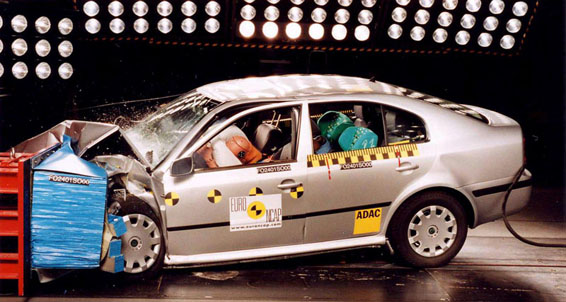
\includegraphics[scale=0.3]{Skoda_Krocktest_27207.png}
\end{figure}
\end{block}
\end{frame}

%Mekanik
\section{Mekanik}
\begin{frame}
\frametitle{Hållfasthet}
\begin{block}{Normalspänning och töjning}
\begin{figure}
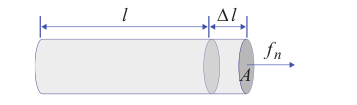
\includegraphics[scale=0.5]{a88-muller.png}
\end{figure}
\begin{itemize}
\item Hookes lag:
\end{itemize}
\begin{equation}
\frac{F_n}{A} = E \frac{\Delta l}{l}
\end{equation}
\end{block}
\end{frame}

\begin{frame}
\frametitle{Hållfasthet}
\begin{block}{Utökning till tre dimensioner}
\begin{itemize}
\item I tre dimensioner beror normalspänning och töjning på mätrikting
\item Skalärrepresentation inte längre tillräckligt, vi använder tensor istället
\item Töjningstensorn kan ställas upp som:
	\begin{equation}
		\epsilon = \nabla \mathbf{u} + \nabla \mathbf{u}^T + \nabla \mathbf{u}^T \nabla \mathbf{u}
	\end{equation}
\item Hookes lag kan då omdefinieras som:	
	\begin{equation}
		\sigma = E \cdot \epsilon
	\end{equation}
\end{itemize}
\end{block}
\end{frame}

\begin{frame}
\frametitle{Hållfasthet}
\begin{block}{Isotropa och anisotropa material}
\begin{itemize}
\item E är kopplingen mellan normalspänning och töjning och definierar materialets egenskaper
\item Isotropa material har samma egenskaper i alla riktningar, till skillnad från anisotropa material som exempelvis trä
\item E för isotropa material kan ställas upp som:
\begin{tiny}

\begin{eqnarray}\label{eqn:ststhooks}
\left[ \begin{array}{c}
\sigma_{xx} \\
\sigma_{yy} \\
\sigma_{zz} \\
\sigma_{xy} \\
\sigma_{yz} \\
\sigma_{xz} \\
\end{array} \right] = \frac{E}{(1+\nu)(1-2\nu)}
\left[ \begin{array}{cccccc}
1-\nu & \nu & \nu & 0 & 0 & 0\\
\nu & 1-\nu & \nu & 0 & 0 & 0\\
\nu & \nu & 1-\nu & 0 & 0 & 0\\
0 & 0 & 0 & 1-2\nu & 0 & 0\\
0 & 0 & 0 & 0 & 1-2\nu & 0\\
0 & 0 & 0 & 0 & 0 & 1-2\nu\\
 \end{array} \right]
\left[ \begin{array}{c}
\epsilon_{xx} \\
\epsilon_{yy} \\
\epsilon_{zz} \\
\epsilon_{xy} \\
\epsilon_{yz} \\
\epsilon_{xz} \\
\end{array} \right]
\end{eqnarray}

\end{tiny}
\end{itemize}
\end{block}
\end{frame}

%Diskretisering
\section{Diskretisering}
\begin{frame}
\frametitle{Finita elementmetoden}
\begin{block}{Diskretisering}
\begin{itemize}
\item Välkänd numerisk metod för att approximera lösningen av kontinuerliga problem
\item Vi representerar våra finita element som tetrahedrar
\item Fyra noder per tetraheder, tre frihetsgrader per nod
\end{itemize}
\begin{figure}
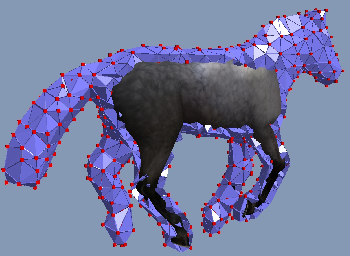
\includegraphics[scale=0.5]{hest.png}
\end{figure}
\end{block}
\end{frame}

\begin{frame}
\frametitle{Finita elementmetoden}
\begin{block}{Diskretisering}
\begin{itemize}
\item Tetrahederstrukturen ger oss en förflyttning per nod
\item Approximationen av det kontinuerliga vektorfältet $\mathbf{u}$ fås som:
	\begin{equation}
		\mathbf{u} \approx N(x,y,z) \hat{u}
	\end{equation}
\item För att utifrån $\hat{u}$ finna töjningstensorn $\epsilon$ använder vi deriveringsoperatorn $L$
	\begin{equation}\label{tio}
    	\epsilon = LN \hat{u} = B_ {e} \hat{u}
	\end{equation}	
\end{itemize}
\end{block}
\end{frame}

\begin{frame}
\frametitle{Finita elementmetoden}
\begin{block}{Styvhetsmatrisen}
\begin{itemize}
\item Utifrån töjningsmatrisen $B_e$ bildar vi den elementvisa styvhetsmatrisen $K_e$:
	\begin{equation}\label{eqn:stiffnessmatrix}
    	K_{e} = V_{e} B_ {e}^{T}EB_ {e}^{T}
	\end{equation}
\item Eftersom varje nod har tre frihetsgrader blir $K_e$ en 12x12-matris som beskriver kopplingarna mellan tetrahederns fyra noder
\item Via Hookes lag får vi kraften per nod som:
	\begin{equation}\label{eqn:stiffnessmatrix}
    	f_{e} = K_ {e}\hat{u}
	\end{equation}
\item För hela systemet bygger vi en global styvhetsmatris, $K$, som beskriver nodernas kopplingar till varandra
\item Eftersom alla noder inte är kopplade till alla blir matrisen $K$ gles
\end{itemize}

\end{block}
\end{frame}


%Systemets dynamik
\section{Systemets dynamik}
\begin{frame}
\frametitle{Systemets dynamik}
\begin{block}{Kraftekvationen}
\begin{itemize}
\item Ansätt Newton's andra lag $\mathbf{f} = m\ddot{\mathbf{x}}$ på de volymetriska elementen. Eftersom att de är obegränsat små och inte har en massa definierad får man dividera ekvationens båda sidor med dess volym.
\item Den totala kraften, $\rho \ddot{x}$, är summan av den inre och den yttre kraften, $f_{ext}$
	\begin{equation}
		\rho \ddot{x} = \mathbf{f}_{ext} + \mathbf{f}_{in}
	\end{equation}
		
\end{itemize}	
\end{block}
\end{frame}


\begin{frame}
\frametitle{Systemets dynamik}
\begin{itemize}
\item Vi ersätter densiteten med en massmatris, $M$, och lägger till dämpning, $C$:
	\begin{equation}
		\mathbf{M\ddot{x}} + \mathbf{C\dot{x}} + \mathbf{K(x - x_0)}  = \mathbf{f}_{ext}
	\end{equation}


\begin{center}
\begin{tabular}{c l}
$\mathbf{M}$ & Massmatris \\
$\mathbf{C}$ & Dämpningsmatris \\
$\mathbf{K}$ & Styvhetsmatris\\
$\mathbf{f}$ & Krafter som verkar på systemet \\
\end{tabular}
\end{center}
\item Vi använder proportionell dämpning, och bildar dämpningsmatrisen $\mathbf{C}$:
	\begin{equation}
		\mathbf{C} = \alpha \mathbf{M} + \beta \mathbf{K}
	\end{equation}

\end{itemize}
\end{frame}

%Integrering
\section{Integrering}
\begin{frame}
\frametitle{Integrering}
\begin{block}{Explicit integrering}
\begin{itemize}
\item Intuitiv implementering
\item Stabilitetsproblem, ackumulering av fel
\end{itemize}
\end{block}

\begin{block}{Implicit integrering}
\begin{itemize}
\item Ovillkorligt stabil
\item Kräver invertering av stor matris
\end{itemize}
\end{block}

\end{frame}

\begin{frame}
\frametitle{Integrering}
\begin{block}{Lösning med implicit Eulerintegrering}
\begin{itemize}
\item Vi vill lösa:
	\begin{equation}
		(\mathbf{M} + \Delta t  \mathbf{C} + \Delta t^2 \mathbf{K})v^{t+1} = \mathbf{M} v - \Delta t (\mathbf{K}(x - x_0) + f_{ext})
	\end{equation}
för $v^{t+1}$
\item Detta är ett linjärt system på formen $Ax = b$
\item Matrisen $\mathbf{K}$ har dimensionen 3n x 3n, där n är antalet noder \begin{tiny}(alltså ganska stor)\end{tiny}, men är lyckligtvis gles.
\item Vi kan använda konjugatgradientmetoden för att approximera en lösning
\item Den resulterande hastigheten används för att uppdatera nodernas position
\end{itemize}
\end{block}
\end{frame}

\begin{frame}
\frametitle{Integrering}
\begin{block}{Konjugatgradientmetoden}
\begin{itemize}
\item Iterativ numerisk metod
\item Matrisen $\mathbf{A}$ gles och symmetrisk
\item Lämplig för vår applikation
\item Vi använder en existerande implementation
\end{itemize}
\end{block}
\end{frame}

%Rendering
\section{Rendering}
\begin{frame}
\frametitle{Rendering}
\begin{block}{Tetrahedermesh}
\begin{itemize}
\item Datastruktur bestående av \texttt{Vertex}, \texttt{HalfEdge}, \texttt{Face} och \texttt{Tetrahed}
\item Metoder för traversering av strukturen och åtkomst av olika typer av data
\item En \texttt{Vertex} har en position, som uppdateras med den framräknade hastigheten
\item Vi kan läsa in olika objekt, i form av en lista med vertexpositioner och en som beskriver vilka vertexar som tillhör vilken tetraheder

\end{itemize}
\end{block}
\end{frame}

%Förbättringar
\section{Förbättring av modellen}


\begin{frame}
\frametitle{Rotations kompensering}

\begin{itemize}
\item Cauchy linjära töjnings tensor är ej rotations invariant vilket gör att styvhets matrisen $K_{e}$ inte gäller då tetraheden roterats från sitt viloläge 

\item Artifakter i form av växande volym

\item Problemet löses genom att extrahera rotationen för varje element mellan viloläget och det deformerade tillståndet

\item $A$ beskriver mappningen mellan de båda tillstånden exklusive translation

\begin{equation}\label{eqn:stiffnessmatrix}
    A = [x_{1}-x_{0}, x_{2}-x_{0}, x_{3}-x_{0}][p_{1}-p_{0}, p_{2}-p_{0}, p_{3}-p_{0}]^{-1}
\end{equation}

\item Gram-smiths metod används för att extrahera rotationen ur $A$
\end{itemize}
\end{frame}

\section{Förbättring av modellen}


\begin{frame}
\frametitle{Rotations kompensering}
\begin{block}{Interna kraften per element}
\begin{itemize}
\item Den interna kraften rotations kompenseras och beräknas som: 
\end{itemize}
\begin{equation}\label{eqn:stiffnessmatrix}
    f_{warped} = R_{e}K_{e}(pR_{e}^{-1}-x)
\end{equation}
\begin{figure}
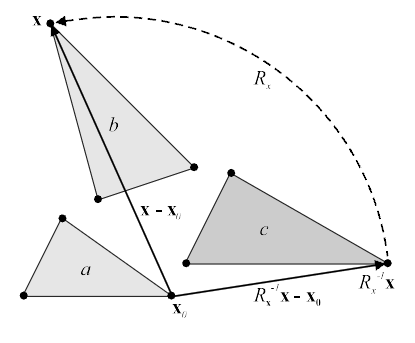
\includegraphics[scale=0.5]{warpedstiffness.png}
\end{figure}
\end{block}
\end{frame}

\section{Förbättring av modellen}
\begin{frame}
\frametitle{Frakturer}
\begin{itemize}
\item Ett material som utsätts för stress kan spricka 

\item Stress tensorn per tetrahed beräknas enligt:
\begin{equation}\label{eqn:stiffnessmatrix}
    \sigma = EB_{e}\hat{u}
\end{equation}

\item Egenvärdesanalys på $\sigma$

\item Välj ut största positiva egenvärdet med motsvarande egenvektor

\end{itemize}
\end{frame}

\section{Förbättring av modellen}
\begin{frame}
\frametitle{Frakturer}
\begin{itemize}
\item Välj en slumpmässig nod i vald tetrahed och spänn upp ett plan genom punkten med egenvektorn som normal

\item Välj ut alla grann tetraheder till noden och kolla om deras masscentrum ligger på planets positiva eller negativa sida

\item Skapa spricka genom frikoppla tetrahederna till två noder enligt bilden

\begin{figure}
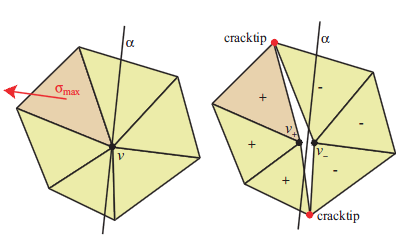
\includegraphics[scale=0.5]{fracture.png}
\end{figure}

\end{itemize}
\end{frame}









\end{document} 